\subsection{Line-line picking}
\label{sec:line_line}

In the simplest case, two points are chosen IID uniformly from a line
of length $L$. 

Figure~\ref{fig:line_pdf} shows the PDF and CDF for the line-line
picking problem.

\begin{figure}[tbp]
  \begin{center}
    \subfloat[\label{fig:line_pdf}PDF of length 1 line.]
       {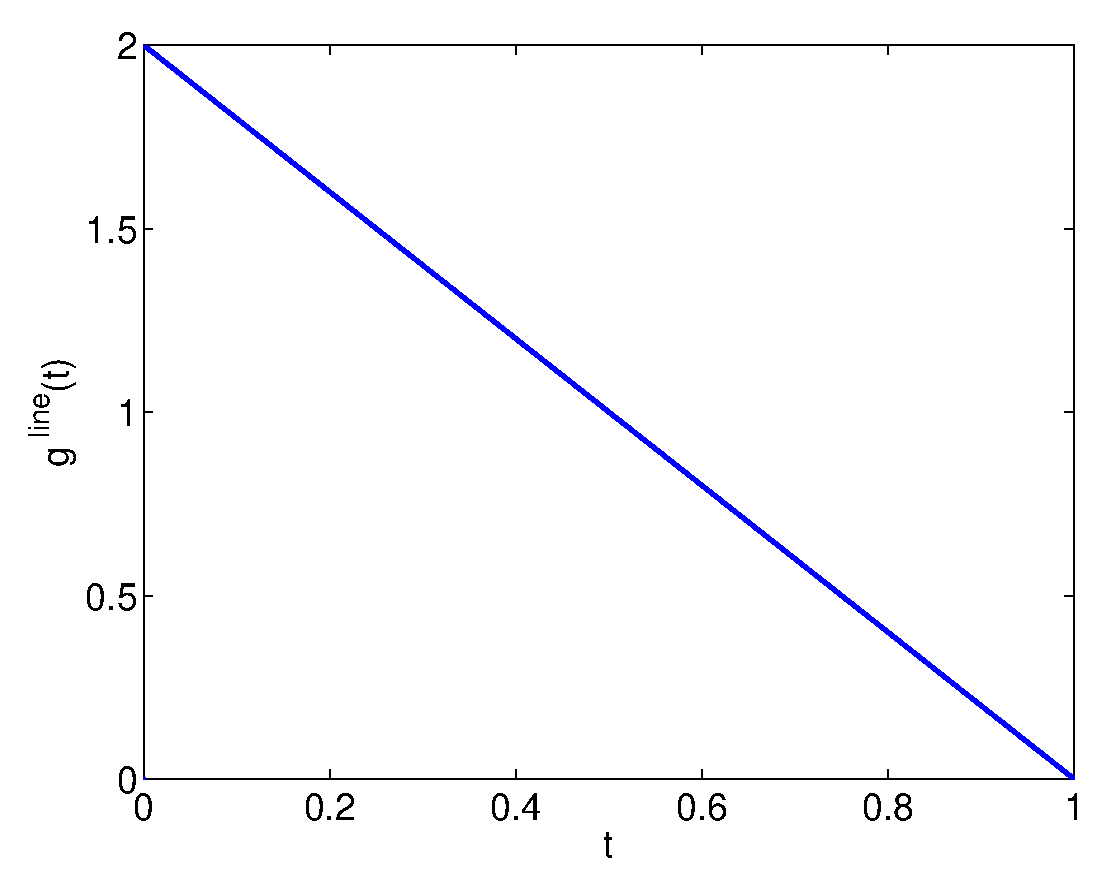
\includegraphics[width=0.48\columnwidth]{../Matlab/Plots/LinePicking_plot_line_pdf.eps}}
    \subfloat[\label{fig:line_cdf}CDF of length 1 line.]
       {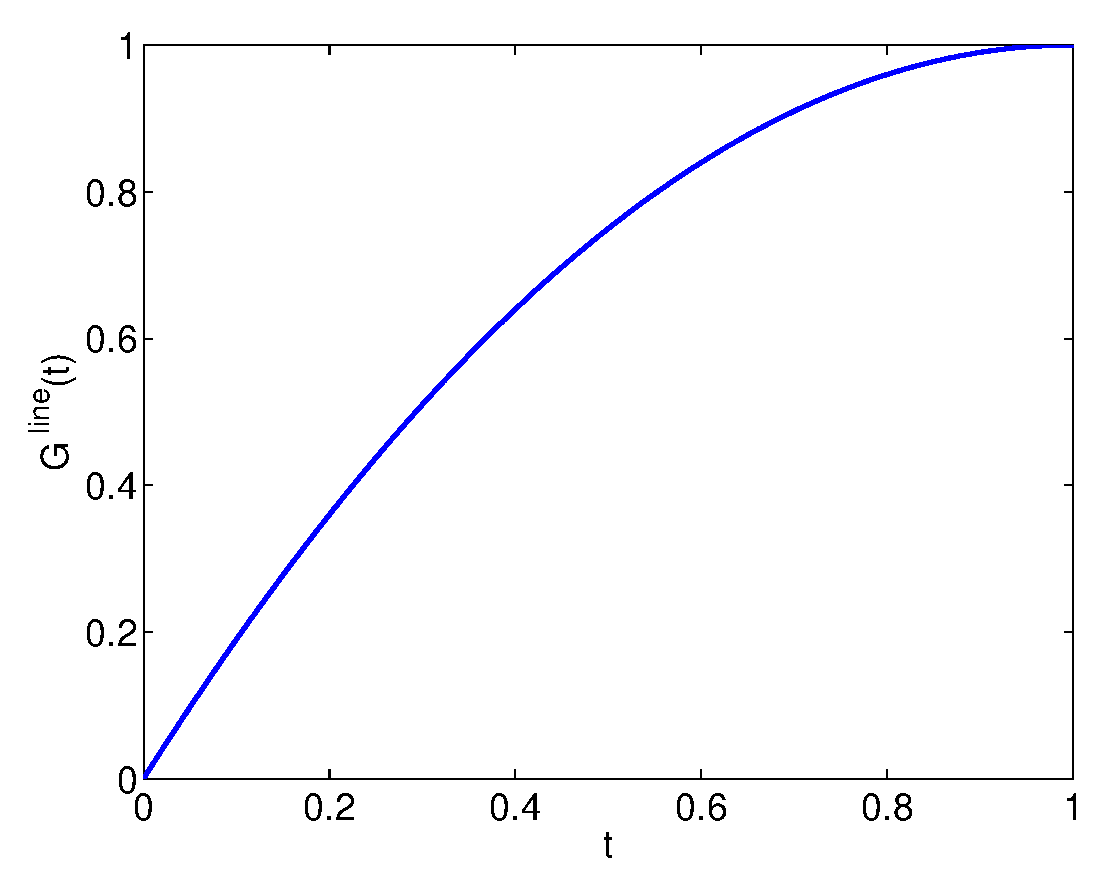
\includegraphics[width=0.48\columnwidth]{../Matlab/Plots/LinePicking_plot_line_cdf.eps}}
    \caption{The line-line picking problem ($L=1$).}
  \end{center}
\vspace{-4mm}
\end{figure}

\subsubsection{PDF}

The probability density function of distances between two (uniformly)
randomly chosen points on the unit line is given in
\cite{weisstein:_line_line_picking,b.ghosh51:_random_rect}, as
\begin{equation}
  \label{eq:line_line}
  g^{\rm line}(t) = 2(1-t),
\end{equation}
or for a line of length $L$ as
\begin{equation}
  \label{eq:line_lineL}
  g^{\rm line}_L(t) = \frac{2}{L} \left( 1-\frac{t}{L} \right).
\end{equation}

This also arises as the limit as $a \rightarrow 0$ for the PDF for the
rectangle \eqref{eqn:rectangle}.

\subsubsection{CDF}

The CDF can be obtained by simple integration:
\begin{eqnarray}
  G^{\rm line}_L(t)
     & = & \int_0^t g^{\rm line}_L(s) \, ds, \nonumber \\
     & = & \frac{2}{L} \int_0^t  1-\frac{s}{L} \, ds, \nonumber \\
     & = & \frac{2}{L} \left[ s - \frac{s^2}{2L} \right]_0^t, \nonumber \\
     & = &  \frac{2}{L} t - \frac{t^2}{L^2}. \\
  \label{eq:line_cdf}  
\end{eqnarray}

\subsubsection{Moments}

The moments are
\begin{eqnarray}
  \alpha_i & = & \int_0^L s^i g^{\rm line}_L(s) \, ds, \nonumber \\
           & = & \frac{2}{L}  \int_0^L s^i- \frac{s^{i+1}}{L}  \, ds, \nonumber \\
           & = & \frac{2}{L} \left[ \frac{s^{i+1}}{i+1} - \frac{s^{i+2}}{L(i+2)} \right]_0^L, \nonumber \\
           & = & \frac{2 L^{i}}{i+1} - \frac{2 L^{i}}{(i+2)}, \nonumber \\
           & = & \frac{2 L^{i} (i+2) - 2 L^{i}(i+1)}{(i+1)(i+2)} , \nonumber \\
           & = & \frac{2 L^{i}}{(i+1)(i+2)} , \nonumber \\
  \label{eq:line_moments}
\end{eqnarray}
Hence the mean and variance are
\begin{eqnarray}
  \mu^{\rm line} & = & \frac{L}{3}, \\
  \label{eq:line_mean}
  \sigma^2_{\rm line}
      & = & \frac{2 L^{2}}{12} - \frac{L^2}{9}, \nonumber \\
      & = & \frac{6 L^{2} -4 L^2}{36}, \nonumber \\
      & = & \frac{L^{2}}{18}.
  \label{eq:line_var}
\end{eqnarray}


